\section{Serial\-Console Class Reference}
\label{classSerialConsole}\index{SerialConsole@{SerialConsole}}
{\tt \#include $<$Serial\-Console.h$>$}

Inheritance diagram for Serial\-Console::\begin{figure}[H]
\begin{center}
\leavevmode
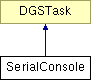
\includegraphics[height=2cm]{classSerialConsole}
\end{center}
\end{figure}
\subsection*{Public Member Functions}
\begin{CompactItemize}
\item 
{\bf Serial\-Console} ()
\item 
{\bf $\sim$Serial\-Console} ()
\item 
virtual int {\bf svc} ()
\item 
int {\bf set\-Commands\-Consumer} ({\bf DGSTask} $\ast$consumer)
\item 
virtual int {\bf Is\-Alive} ()
\end{CompactItemize}


\subsection{Detailed Description}
Provides console like access to the serial port. 



\subsection{Constructor \& Destructor Documentation}
\index{SerialConsole@{Serial\-Console}!SerialConsole@{SerialConsole}}
\index{SerialConsole@{SerialConsole}!SerialConsole@{Serial\-Console}}
\subsubsection{\setlength{\rightskip}{0pt plus 5cm}Serial\-Console::Serial\-Console ()}\label{classSerialConsole_a0}


Serial\-Console constructor \index{SerialConsole@{Serial\-Console}!~SerialConsole@{$\sim$SerialConsole}}
\index{~SerialConsole@{$\sim$SerialConsole}!SerialConsole@{Serial\-Console}}
\subsubsection{\setlength{\rightskip}{0pt plus 5cm}Serial\-Console::$\sim${\bf Serial\-Console} ()}\label{classSerialConsole_a1}


{\bf Serial\-Console::$\sim$Serial\-Console}{\rm (p.\,\pageref{classSerialConsole_a1})} Destructor 

\subsection{Member Function Documentation}
\index{SerialConsole@{Serial\-Console}!IsAlive@{IsAlive}}
\index{IsAlive@{IsAlive}!SerialConsole@{Serial\-Console}}
\subsubsection{\setlength{\rightskip}{0pt plus 5cm}virtual int Serial\-Console::Is\-Alive ()\hspace{0.3cm}{\tt  [inline, virtual]}}\label{classSerialConsole_a4}


Is\-Alive Prints a messages signaling that is alive

\begin{Desc}
\item[Returns:]\end{Desc}


Reimplemented from {\bf DGSTask} {\rm (p.\,\pageref{classDGSTask_a1})}.\index{SerialConsole@{Serial\-Console}!setCommandsConsumer@{setCommandsConsumer}}
\index{setCommandsConsumer@{setCommandsConsumer}!SerialConsole@{Serial\-Console}}
\subsubsection{\setlength{\rightskip}{0pt plus 5cm}int Serial\-Console::set\-Commands\-Consumer ({\bf DGSTask} $\ast$ {\em consumer})\hspace{0.3cm}{\tt  [inline]}}\label{classSerialConsole_a3}


set\-Commands\-Consumer Set the pointer to the Serial handler accepting console messages

\begin{Desc}
\item[Parameters:]
\begin{description}
\item[{\em consumer}]The pointer to the hander implementing a message queue that can be used to input messages using the \char`\"{}put\char`\"{} function\end{description}
\end{Desc}
\begin{Desc}
\item[Returns:]\end{Desc}
\index{SerialConsole@{Serial\-Console}!svc@{svc}}
\index{svc@{svc}!SerialConsole@{Serial\-Console}}
\subsubsection{\setlength{\rightskip}{0pt plus 5cm}int Serial\-Console::svc ()\hspace{0.3cm}{\tt  [virtual]}}\label{classSerialConsole_a2}


svc Internal console loop. Read keyboar commands

\begin{Desc}
\item[Returns:]\end{Desc}


The documentation for this class was generated from the following files:\begin{CompactItemize}
\item 
{\bf Serial\-Console.h}\item 
{\bf Serial\-Console.cpp}\end{CompactItemize}
